\documentclass[10pt,twocolumn,letterpaper]{article}

\usepackage{statcourse}
\usepackage{times}
\usepackage{epsfig}
\usepackage{graphicx}
\usepackage{amsmath}
\usepackage{float}
\usepackage{amssymb}
\usepackage{lipsum}


\usepackage[breaklinks=true,bookmarks=false]{hyperref}


\statcoursefinalcopy


\setcounter{page}{1}
\begin{document}


\title{Electricity Demand Forecasting using  LSTM-based RNNs in Romania}


\author{Apolline Foucher\\
{\tt\small a.foucher@mpp.hertie-school.org}
\and
Augustine Malija\\
{\tt\small a.malija@mpp.hertie-school.org}
\and
Vlad Surdea-Hernea\\
{\tt\small v.surdea-hernea@mpp.hertie-school.org}
}


\maketitle
%\thispagestyle{empty}



% MAIN ARTICLE GOES BELOW
%%%%%%%%%%%%%%%%%%%%%%%%%%%%%%%%%%%%%%%%%%%%%%%%%%%%%%%%%%%%%%%


%%%%%%%%% ABSTRACT
\begin{abstract}
 Electricity demand forecasting is the central challenge for the operators of a modern grid system. Traditionally, this computational problem has been tackled using statistical models such as the Autoregressive Integrated Moving Average (ARIMA)  model. However, recent developments show that machine-learning methods, especially ones employing deep-learning architectures, outperform the traditional econometric models. In this paper\footnote{GitHub account \url{https://github.com/vladsurdea/ML}}, we conduct a series of experiments to demonstrate that a LSTM-based RNN is capable of forecasting accurately the complex electric load time series, even in the absence of weather-related data. We show that the performance of the deep-learning approach compares favorably to the ARIMA model, regardless of the metric used for assessment. 
\end{abstract}


%%%%%%%%% BODY TEXT
\section{Introduction}

\subsection{Background}
The deep decarbonization of the European Union’s economic sectors implies the massive electrification of industry, transport, and heating and cooling. Additionally, the rapid growth of the renewable energy sources (RES) share in the energy mix comes with its own organic challenges, such as seasonal and technology-specific intermittencies.  Overall, the upcoming decades will bring the urgent need to reform and smarten the electricity grid, making it capable of serving the contemporary needs of the European Union member states in a sustainable manner. To enable the well-functioning of this smart grid, operators in the distribution and transport phases of electricity production will have to improve their capacity to predict electricity loads well in advance. Therefore, electricity demand forecasting (EDF) lies at the foundation of the EU’s decarbonization plans, being essential for the management of the national electricity market. 

EDF is a primary input in decisions ensuring the security of energy supply, as well as the optimal requirements for adjacent markets such as the electricity balancing market. Mistakes related to EDF can lead to significant societal problems:

\begin{itemize}
\item	Overestimating daily electricity demand can lead to the waste of resources, introduces unnecessary pressure on the environment through the extra-functioning of fossil-fuel-powered plants and could ultimately prevent the optimal deployment of new renewable sources of electricity production. 
\item Underestimating electricity demand is also a significant issue, as it can lead to prolonged blackouts, or introduce supplementary costs for the participants in the electricity market who would need to pay the higher tariffs existing on the balancing markets.
\end{itemize}

In the past, EDF was primary realized through the usage of traditional econometric models such as the auto-regressive (AR) method, exponential smoothing (ES) method, and auto-regressive moving average (ARIMA) method. The main disadvantage of all the previously-mentioned models it the assumption that past load changes will continue until the present with an identical trend. Given the non-linearity of electricity loads across time and across space, especially in the case of residential electricity consumption, this assumption is rather strong and unlikely to reflect properly the realities of the electricity sectors. Thus, traditional time series statistical models have failed to improve their accuracy during the last decades, leading to the previously described problems. This is the primary reason for which machine-learning models have gained traction in recent years, especially since the rise of renewable energy. 

\subsection{Research Scope}

In this project we deploy deep-learning architectures, in the form of Long Short-Term Memory (LSTM)-based Recurrent Neural Networks (RNNs) to solve the challenge of EDF. To precisely characterize the accuracy of our model, we compare and contrast it with the results of a traditional ARIMA model applied to the same dataset. The proposed LSTM-based RNN exploits long-term dependencies in the electricity consumption time series for generating accurate forecasting of the aggregate load. 

Because there was no previous similar research applied for Eastern Europe, and because recently there was a rise of consultancy companies using machine learning models for EDF in this region, we chose to focus on the Romanian market. Therefore, this paper applies LSTM-based RNNs to the challenge of EDF in Romania.


\subsection{Structure of the Project}
The remainder of this paper is organized as follows:
\begin{itemize}
    \item Section 2 briefly reviews the literature in the field, emphasizing the efficiency and effectiveness of using LSTM-based RNNs for EDF.
    \item Section 3 presents our methodological setup, including mathematical descriptions of both the ARIMA and LSTM-based RNN, as well as the coding strategy of this project.
    \item Section 4 and 5 describe the experiments we have conducted and analyses the results obtained through them.
    \item Section 6 concludes this paper.
\end{itemize}





\section{Related Work}

Given the rapid and significant advancements of machine-learning, in particular deep-learning, researchers have utilized different multiple architectures for a plethora of EDF challenges. Different time resolutions have been studied for several time intervals: monthly, weekly, daily, hourly, half-hourly, minute-by-minute. These deep-learning architectures have been used to target different markets such as business consumers, household consumers,industrial consumers, etc. Thus, our proposed model of applying LSTM-based RNNs to EDF in Romania is based in the latest literature in the field, as represented by papers such as the following:

\begin{itemize}

\item Lago et al.(2018) propose a novel machine-learning
approach towards EDF on the spot market. In order to prove the effectiveness of their methodology, the authors compare and contrast 27 state-of-the-art models used in academia and industry. They prove that in general, any type of machine-learning model outperforms the standard statistical models, and in particular the LSTM-based RNN approach tends to yield very accurate results. The LSTM-RNN approach is the most accurate in cases in which the expected load is not linear, which is mostly the case in the retail market.

\item  Zheng et al. (2017) use LSTM-based RNN in order to manage the nonlinear, non-stationary and nonseasonal nature of the electric load time series. The authors use 906 different samples and train their model such that it predicts the load in the next day based on the given loads from the past ten days. Multiple experiments show that LSTM-based RNNs outperform traditional methods of EDF, especially in the case of short-terms EDF, which is the hardest to predict using statistical tools.

\item Muzaffar and Afshari (2019) find that regardless of the
horizon for the prediction (next day, next hour, next month, etc.), LSTM-based RNNS outperform traditional statistical models such as SARIMA, ARMA and ARMAX. Having access to a large dataset, the authors train the LSTM-based RNN on the first 12 months of
observation and use the 13th month for testing. One interesting fact discovered by Muzaffar and Afshari(2019) is that over-learning might be an issue for a larger number of hidden units.

\item Son and Kim (2020) apply the same machine-learning
approach to EDF to a dataset spanning 22 years of electrical loads in South Korea. The performance of the LTSM-based RNN has been subjected to a comparison with the 4 standard statistical models, and the performance is assessed using 6 different benchmark criteria (MAE, RMSE, MAPE, C, MBE, and UPA).
While LSTM RNNs outperform other models in all six categories, the authors recognize that different criteria yield different accuracy disparities.


\end{itemize}

\section{Proposed Method}

The following section describes the two models used for EDF in the Romanian market. We firstly describe, briefly, the mathematical foundations of the traditional ARIMA model, and afterwards we move towards a comprehensive analysis of the architecture of LSTM-based RNNs.

\subsection{Baseline Model: ARIMA}

ARIMA is the most well-known statistical method created for time series analysis, used primarily  to forecast univariate data. This model is defined by three central factors: p, d, and q .These represent the auto-regressive average factor, the integration average factor, and the moving average factor. The mathematical expressions of the model is detailed below: 

$$\Phi_p(BO)(1-BO)^{d}Y_t=\Theta_q(BO)e_t+\delta$$

where $\Phi$ indicates the auto-regressive parameter of order p, p indicates the number of auto-regressive terms in the time series, BO represents the backshift operator, d indicates the number of non-seasonal differences in the series, $Y_t$ indicates the actual value in the  time series data at moment t, $\Theta_t$ is the order p’s auto-regressive parameter at moment t, q indicates the number of forecasting errors, which are lagged in the forecasting equation, $e_t$ is a random perturbation or white noise for each moment t, and $\delta$ indicates a constant value.



\subsection{LSTM-based RNN}

In standard RNN architectures, the neural network is designed as a chain of identical modules formed as a series of hidden networks, usually in the form of a single sigmoid layer (see Figure 1). Given that the architecture of an RNN assigns one layer for each moment in time, it is theoretically suitable for time series analysis. However, training  sequences with very long time steps is challenging due to the RNN’s inherent limitations,such as  vanishing gradients.

\begin{figure}[h]
   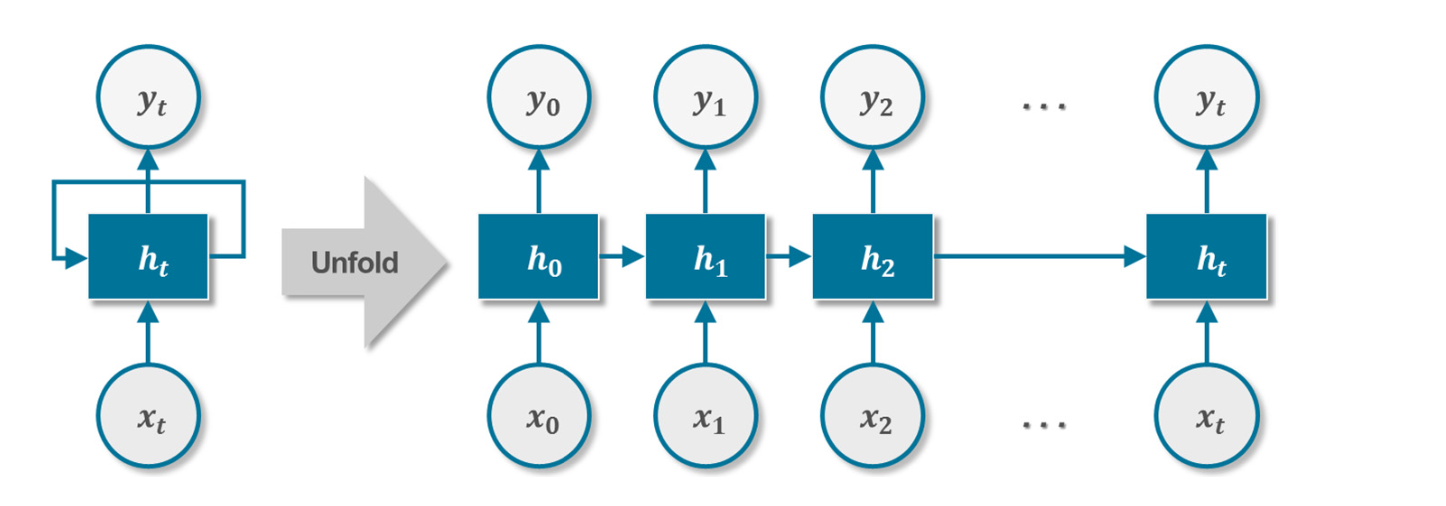
\includegraphics[width=\linewidth]{RNN}
   \caption{The standard architecture of RNNs}
\end{figure}

In contrast to this standard architecture, the hidden layers of a LSTM-based RNN have a more complex structure capable of learning long-term dependencies. The LSTM-extension introduces the concepts of gate and memory cell in each hidden layer in the network. As a consequence, a memory block in the LSTM-based RNN is composed of four structural parts: an input gate , a forget gate , an output gate , and the self-connected memory cells:
\begin{itemize}
    \item The input gate manages the entry of the activations to the memory cells of the neural network.
    \item The output gate is designed to learn what cell activations to filter and, therefore, send as output to the successive network.
    \item The forget gate assists the neutral network to disregarding the past input data and reset the memory cells for the new inputs.
\end{itemize}
In addition to this tripartite structure, LSTM applies multiplicative gates to make it possible for the memory cells to access and store the information over a long time interval.


Briefly stated, based on the input time-series vector \textbf{x}=$\{x_1,x_2,x_3,...x_t\}$, the LSTM-based RNN will predict sequences: the hidden state sequence  \textbf{y}=$\{y_1,y_2,y_3,...y_t\}$ and the output sequence \textbf{h}=$\{h_1,h_2,h_3,...h_t\}$.The process is iterative, and is realised by sequentially updating the states of the memory cells.This process if illustrated in Figure 2, and subsequently described through a series of equations:

\begin{figure}[h]
\begin{center}
    
   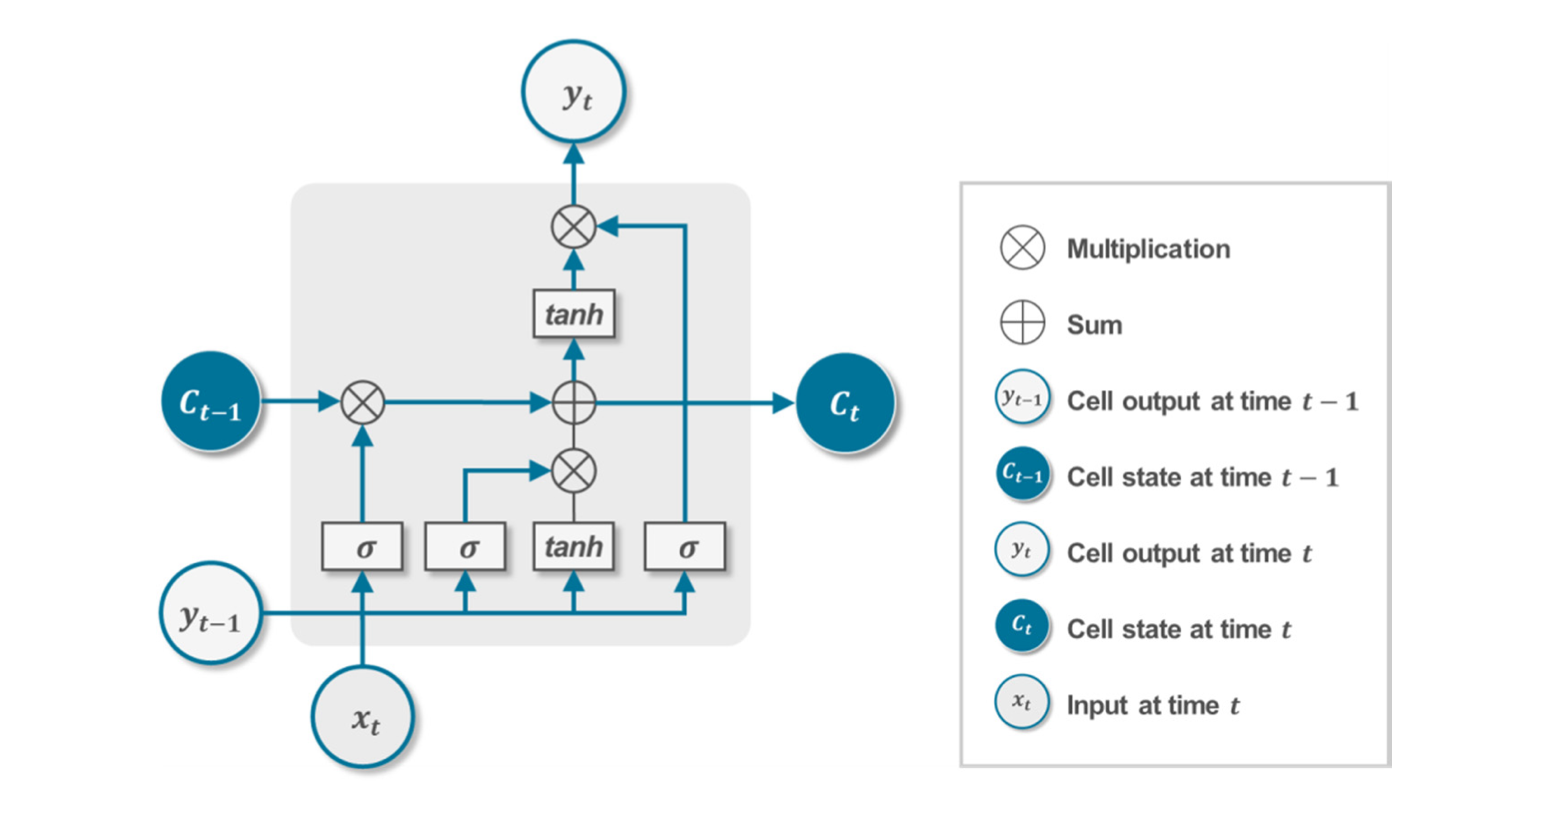
\includegraphics[width=10cm]{final-report-latex/LSTM.png}
   \caption{The long short-term memory (LSTM)-based RNN architecture}
   \end{center}
\end{figure}

The first step in the process is for the forget gate to be applied in order to decide what part of the information to discard from the cell state.The activation of the forget gate is computed via the use of a sigmoid function:

$$f_t=\sigma(W_{ix}x_t+ W_{fw}h_{t-1}+W_{fc}C_{t-1}+b_f) $$

 $f_t$ has values between 0 and 1, where 0 would mean discarding all the information from the last cell state, and 1 retaining all the information in the last cell state. Nevertheless, usually the value does not attain this extreme values.
 
After deciding what information to forget, the LSTM model decides what new information to store in the new cell state. Once again, a sigmoid function is used to determine the input gate layer. This second step is the reverse, symmetrical operation to the first step.

$$i_t=\sigma(W_{ix}x_t+W_{ih}h_{t-1}+W_{ic}C_{t-1}+b_i)$$

Potential values of the new cell states are included in a new vector, $U_t$, that is computed by using the standard sigmoid layer present in the RNN.

$$U_t=g(W_{cx}x_t+W_{ch}h_{t-1}+W_{ic}C_{t-1}+b_i) $$

The old cell state $C_{t−1}$ is updated to a new cell state $C_t$, with the support of the previously-estimated $f_t$ and $U_t$. $f_t$ is being used in order to deduce what  information to forget from the last state $C_{t−1}$ , while $U_t$ is used to understand how much new information to retain:

$$C_t=U_ti_t+C_{t-1}f_t $$

Based on this, the output gate is produced using a different sigmoid layer of the network:

$$o_t=\sigma(W_{ox}x_t+W_{oh}h_{t-1}+W_{oc}C_{t-1}+b_o$$

A cell output sigmoid activation function $\ell$ is applied over the cell state, which is then multiplied by the output $o_t$ to generate the desired information about $h_t$:

$$h_t=o_t \ell(C_t) $$

An output activation function $k$is used to produce information about the output of the memory block:

$$y_t=k(W_{yh}h_t+b_y)$$

The sigmoid functions are usually expressed as:

$$\sigma(x)=\frac{1}{1+e^{-x}}$$

The activation functions are usually expressed as:

$$tanh(x)=1- \frac{2}{e^{2x}+1} $$

\subsection{Coding strategy}

The proposed LSTM-based RNN model was implemented using Keras from Tensorflow. This model, consisting of one input layer, five hidden layers and one output layer, was trained with a mean-squared error (MSE) loss function and optimized through adaptive moment estimation (ADAM) optimization scheme. ADAM was chosen instead of rmsprop, which is the other standard alternative. The pre-processing of the data was straightforward, making sure that we obtain a dataset that contains all the time-series information (hour, day, weekday, week, month, year) as well as the value of the electricity load consumed for each of the observations in the time-series. For reasons of clarity, we also introduced a date-time variable as the index of the dataset.

\section{Experiments}

\paragraph{Data:} For the scope of this project, we use the historical electricity consumption database provided by the European Network of Transmission System Operators (ENTSO-E). This database encompasses a range of data-sets provided by national Transmission System Operators (ENTSO-E) in
Europe.

 We have extracted, from the aggregate dataset, data relevant for the case of Romania. This was done in order to explore a market that was previously ignored by researchers trying to compare the accuracy of machine-learning methods with econometric models for the task of EDF. The dataset provided by the Romanian TSO contains 119771 observations, one for each hour between 01.01.2006 and 31.08.2019.

The following set of figure visually characterises the dataset and allows us to draw intermediate conclusions  about what an accurate model would have to account for. Additionally, these figures were presented to the human evaluators, so that they can have a sense of what has been used as input for the LSTM-based RNN.

Figure 3 displays the evolution of electricity demand in the period 2006-2019 in Romania. As we can see, previous years suggest a continuous average increase of the consumed loads. 
The exception is centered around the years 2008 and 2012, which were marked by a financial, respectively political crisis in the country. Since 2013, the average load has been constantly increasing.
\begin{figure}[H]
\begin{center}
   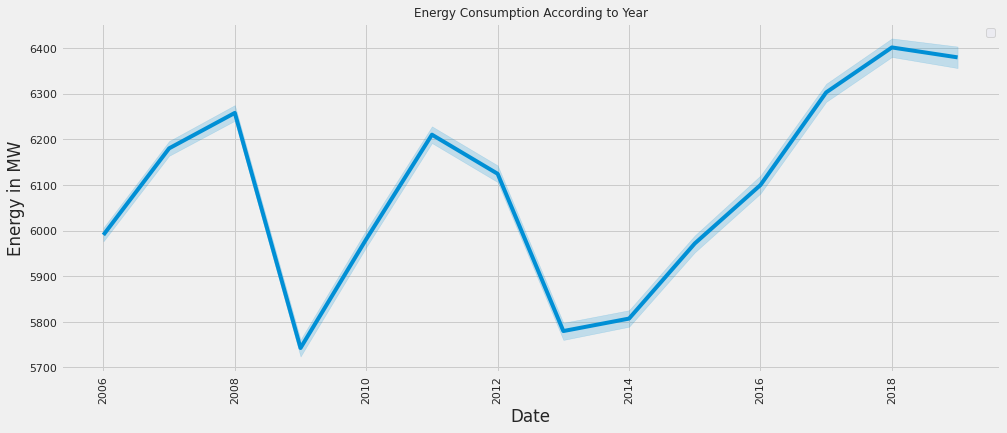
\includegraphics[width=8.5cm]{final-report-latex/Figure1.png}
   \caption{Per year electricity demand in Romania over the period 2006-2019}
   \end{center}
\end{figure}
Figure 4 looks at the distribution of electricity demand across the 12 months. As expected, demand for electricity was significantly higher during winter months and lower during summer, the end of spring and the beginning of autumn.

\begin{figure}[H]
\begin{center}
   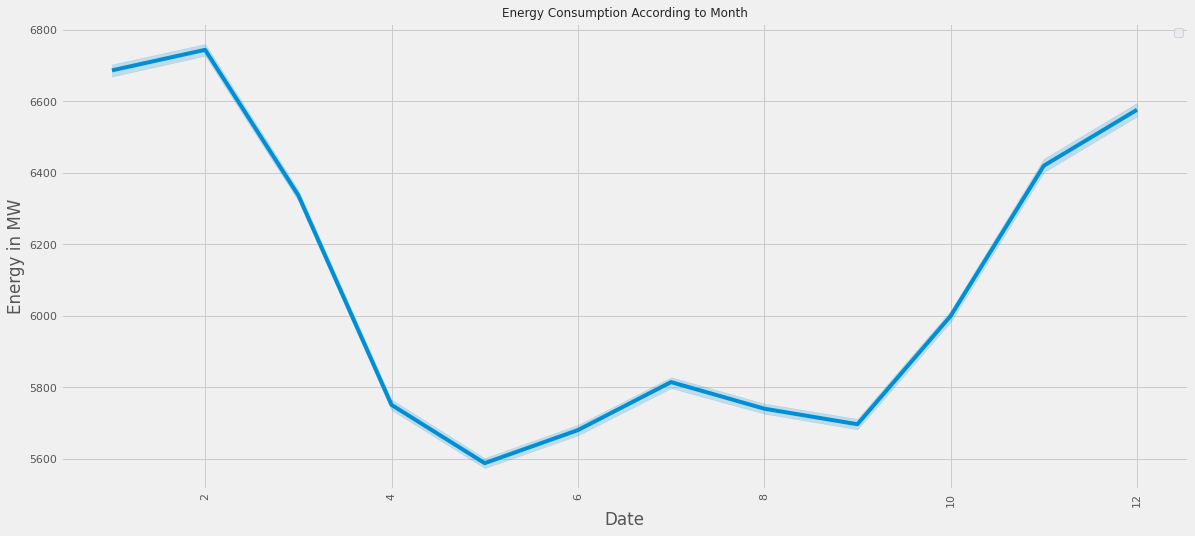
\includegraphics[width=9cm]{final-report-latex/Month.png}
   \caption{Per month electricity demand in Romania over the period 2006-2019}
   \end{center}
\end{figure}

Figure 5 looks at the distribution of electricity demand across the 52 weeks, which captures the same seasonality as the monthly distribution, only more granular.

\begin{figure}[H]
\begin{center}
   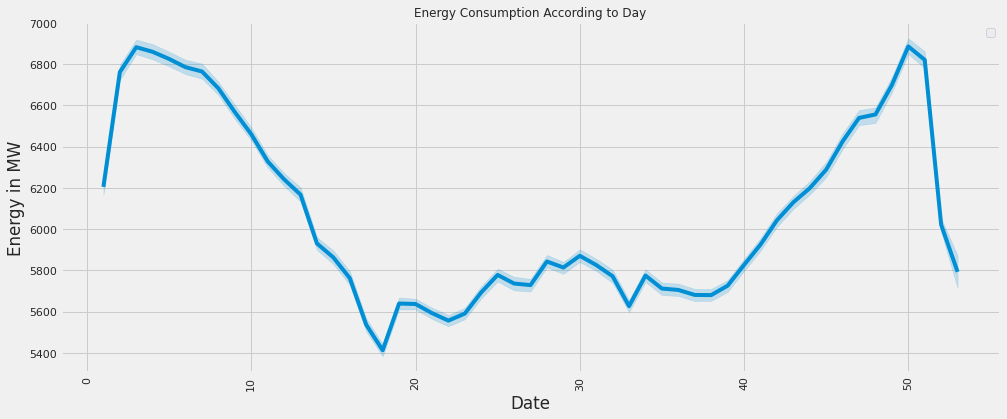
\includegraphics[width=9cm]{final-report-latex/Week.png}
   \caption{Per week electricity demand in Romania over the period 2006-2019}
   \end{center}
\end{figure}

Figure 6 looks at the distribution of electricity demand across the days of the month. Surprisingly, it seems there is also a degree of daily seasonality, as people tend to consume less electricity at the start and end of the month.
\begin{figure}[H]
\begin{center}
   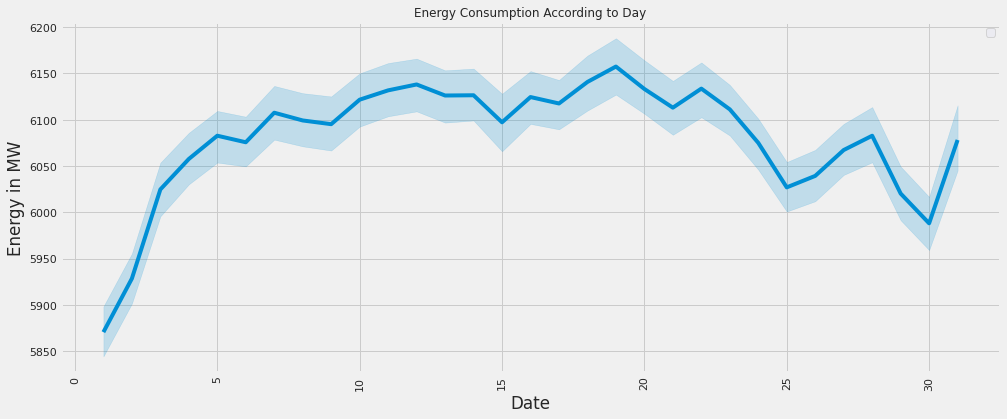
\includegraphics[width=9cm]{final-report-latex/Day.png}
   \caption{Per day electricity demand in Romania over the period 2006-2019}
   \end{center}
\end{figure}

Figure 7 captures the weekday seasonality. Again, as expected, people tend to consume more electricity during weekdays, and significantly less during weekends.

\begin{figure}[H]
\begin{center}
   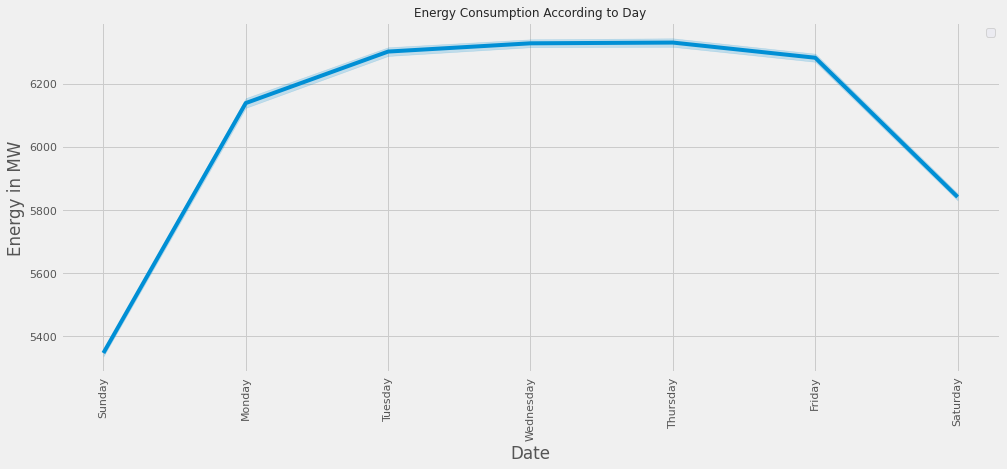
\includegraphics[width=9cm]{final-report-latex/Weekday.png}
   \caption{Per weekday electricity demand in Romania over the period 2006-2019}
   \end{center}
\end{figure}

Figure 8 illustrates the hourly seasonality. In this sense, people clearly use more electricity during day-time. Additionally, the decrease is very steep between the afternoon and the nighttime. 

\begin{figure}[H]
\begin{center}
   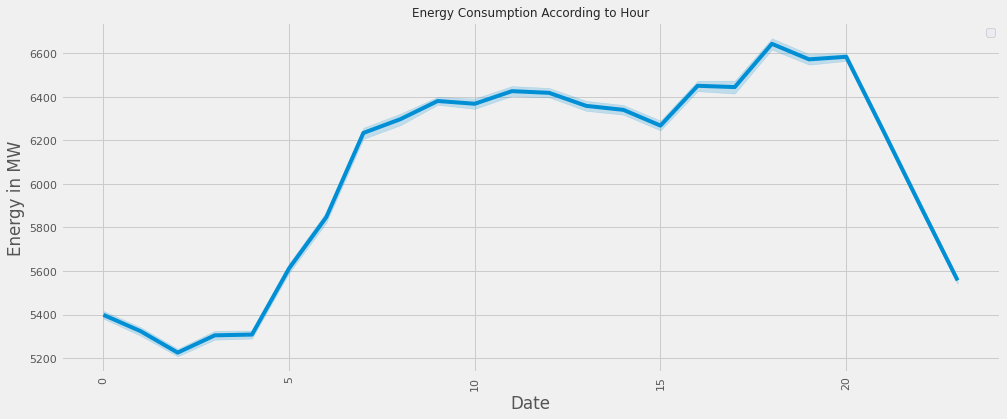
\includegraphics[width=9cm]{final-report-latex/Hour.png}
   \caption{Per hour electricity demand in Romania over the period 2006-2019}
   \end{center}
\end{figure}

Lastly, when looking at Figure 9, one can observe that electricity consumption follow an almost-normal distribution, centered around the mean 6080 MWh and a median of 6050 MWh. This information already provides us with the simplest baseline model, one which would predict for each hour in the testing subset the average 6080 MWh of the entire dataset.


\begin{figure}[h]
\begin{center}
   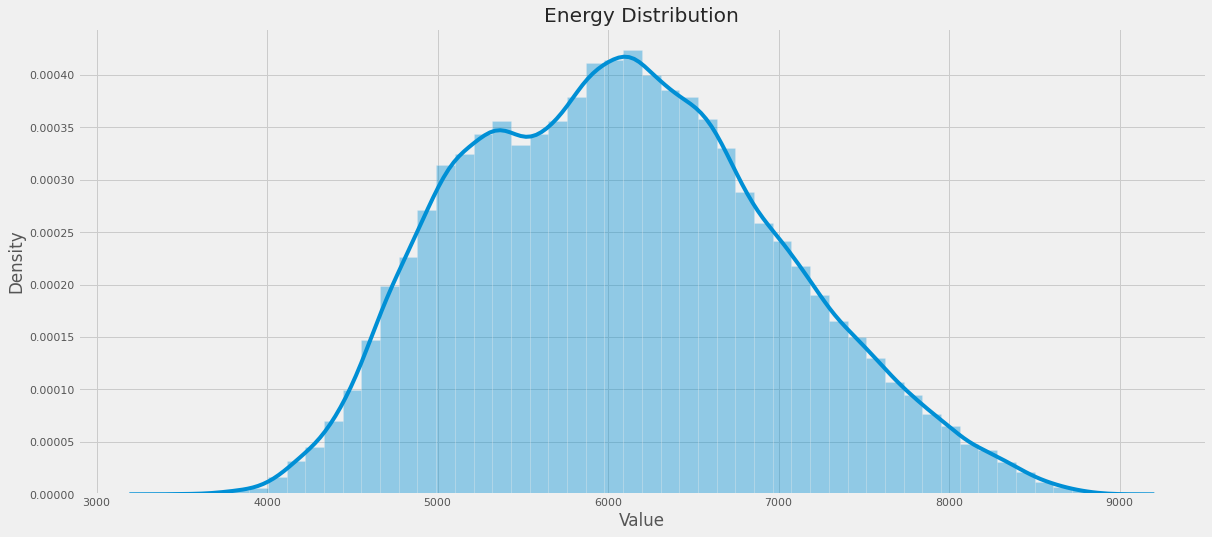
\includegraphics[width=9cm]{final-report-latex/Figure3.png}
   \caption{Distribution of electricity consumption in Romania}
   \end{center}
\end{figure}


\paragraph{Software}: We made use of both Jupyter Lab and Google Colab for writing the code. In terms of managing the project, we benefited from GitHub. Overleaf was the choice for writing the project in \LaTeX.

\paragraph{Hardware}: 
In general, training the deep-learning architecture required the usage of significant GPUs, which was mainly done via Google Col. However, a large number of tests and experiments were also conducted using our personal hardware, listed below:

\begin{itemize}
\item \textbf{Apolline}: Asus, Intel(R) Core(™) i5-8250U CPU @
1.60GHz
\item \textbf{Augustine}: Lenovo T470s, Intel(R) Core(™) i5-7300U
CPU @ 2.60GHz 2.71 GHz, RAM 16GB
\item \textbf{Vlad}: MacBook Pro 2019, 2,3 GHz Quad-Core Intel® Core™ i9 2.30 GHz
\end{itemize}
\paragraph{Evaluation method:} 

The evaluation of the LSTM-model is done using a series of benchmark metrics, used in multiple studies that compare different options for EDF:
\begin{itemize}

\item Mean bias error (MAE) and  Root-mean-squared
error (RMSE), which are absolute performance measures that allow us to compare the deviation between
the actual values and the predictions.

$$ RMSE = \sqrt{\frac{\sum_{i=1}^{n}(x_i-y_i)^2}{n}} $$

$$ MBE= \frac{\sum_{i=1}^{n}(y_i-x_i)}{n} $$

\item MAPE, which is a relative measure that represents the forecasting error between the actual value and the prediction:

$$MAPE=\frac{1}{n}\sum_{i=1}^{n}|\frac{y_i-x_i}{y_i}|100$$

\end{itemize}


\paragraph{Experimental details:} We conducted multiple experiments in the case of the LSTM-based RNN, trying to achieve the best configuration. Ultimately, we observed that using five LSTM layers and fitting a model with 100 epochs and a batch size of 32 was sufficient. In the case of the ARIMA, multiple experiments were not necessary, optimization could only take place by adding additional weather data as inputs, which is beyond the scope and interest of this project.

Furthermore, we experimented with different structures for splitting test and train data. Given that, in practice, EDF involves predicting future values based on the historical time-series, we have always set the last values in the time-series as the testing set.

\paragraph{Results:}

\begin{center}
 \begin{tabular}{||c c c c||} 
 \hline
Evaluation metric & LSTM & ARIMA &\\ [0.5ex] 
 \hline\hline
 MAPE & 0.057 & 234,819.59 &\\ 
 \hline
 MBE & -26.97 & 1,476.66 &\\
 \hline
 RMSE & 602.44 & 2,818.64 & \\
 \hline
\end{tabular}
\end{center}

The table above describes the results of both our baseline ARIMA model, and the LSTM-based RNN model. In this sense, at the first glance, we observe that the LSTM outperforms the traditional model in all categories, so irrespective of the metric used for computing accuracy.


\paragraph{Comment on your quantitative results.} 

Firstly, the comparison with the ARIMA model reveals significant improvements. In practice this would imply massive cost reductions for the companies managing the electricity grid in Romania. The huge improvements measured by the MAPE score are the most important given the scope of this project, as they show that in relative terms, our accuracy would allow for improvements in the electricity balancing market, which is one of the most sensitive and costly elements of the modern electricity grid.



Secondly, the results are better than initially expected, as our model seems to outperform similar models that were also trained using weather-data, not only the electricity load time-series. The absence of weather-data seems to be not so relevant, which is surprising given the history of other papers (including papers that use deep-learning methods). However, this might be explained by the peculiarity of the Romanian market, which is mostly driven by hydro power and nuclear power. Both hydro and nuclear are base-load technologies with extremely low variation capabilities. In this sense, the market generated by these technologies is very different from one in which wind and solar PV would play more significant roles. However, given the expected increase in the role of these renewable sources in Romania in the upcoming decades, it is advisable for deep-learning EDF models to also use weather data as input (if available). Additionally, one can see that the ARIMA model was, in opposition to the LSTM-based RNN, significantly affected by the lack of weather data.

Thirdly, the human evaluators from Romania have revealed one important fact about the results of our model. The negative MBE in the case of the LSTM implies that our approach underestimated the actual electricity consumed by the Romanian markets at a given point in time. While the very small value of the MBE is an improvement from the ARIMA model, negative values are dangerous in EDF. This is because from a grid-operating perspective it is easier to work with overestimated values (and thus with companies producing more, and electricity prices going up) than with underestimated values (and thus with companies producing less, and either prices spiking or blackouts happening). These results indicated that future deep-learning approaches to EDF might need, if also leading to negative MBEs, to be adjusted upwards. The mathematical way of doing this is beyond the scope of this project.


\section{Analysis}

Figure 10 displays the results of the ARIMA model. While the model predicts the direction in which the electricity load seems to go, it is inaccurate in actually determining the load at a given moment.  Given that ARIMA is a traditional econometric model, it doesn't use the train-test split. As such, one can see the predicted values alongside the actual values of the electricity load across the entire dataset. Nevertheless, the results do not improve if we only look at one period in time, as the main fault of the model is the incapacity of anticipating spikes in demand. 

\begin{figure}[H]
\begin{center}
   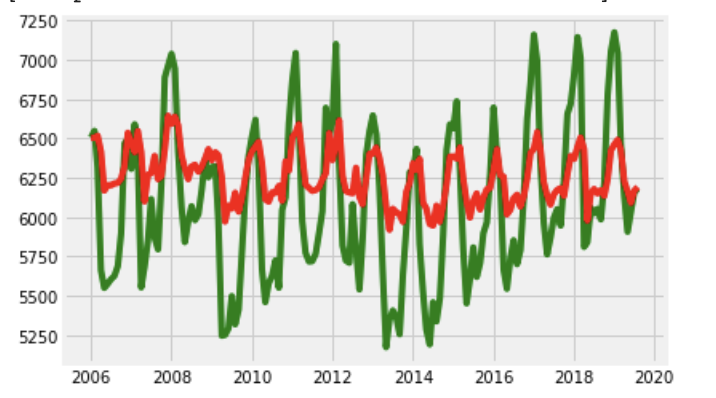
\includegraphics[width=9cm]{final-report-latex/ARIMA_Figure.png}
   \caption{ARIMA model results}
   \end{center}
\end{figure}

Figure 11 displays the results of the LSTM-based RNN model. This plot offers the results of the test aggregate on a daily basis. The improvements from the previous models are visually perceivable. One very important point, however, is that results tend to become better and better as we go towards the end of the dataset. In this sense, one can conclude that the best EDF approach with LSTM-based RNN would be to predict a small number of electricity loads based on a very large pre-existing historical time-series. This is ideal, as usually the most important predictions are for the upcoming day, and at most for the next 7 days. Our prediction for a couple of months is beyond the needs of the industry. 

\begin{figure}[H]
\begin{center}
   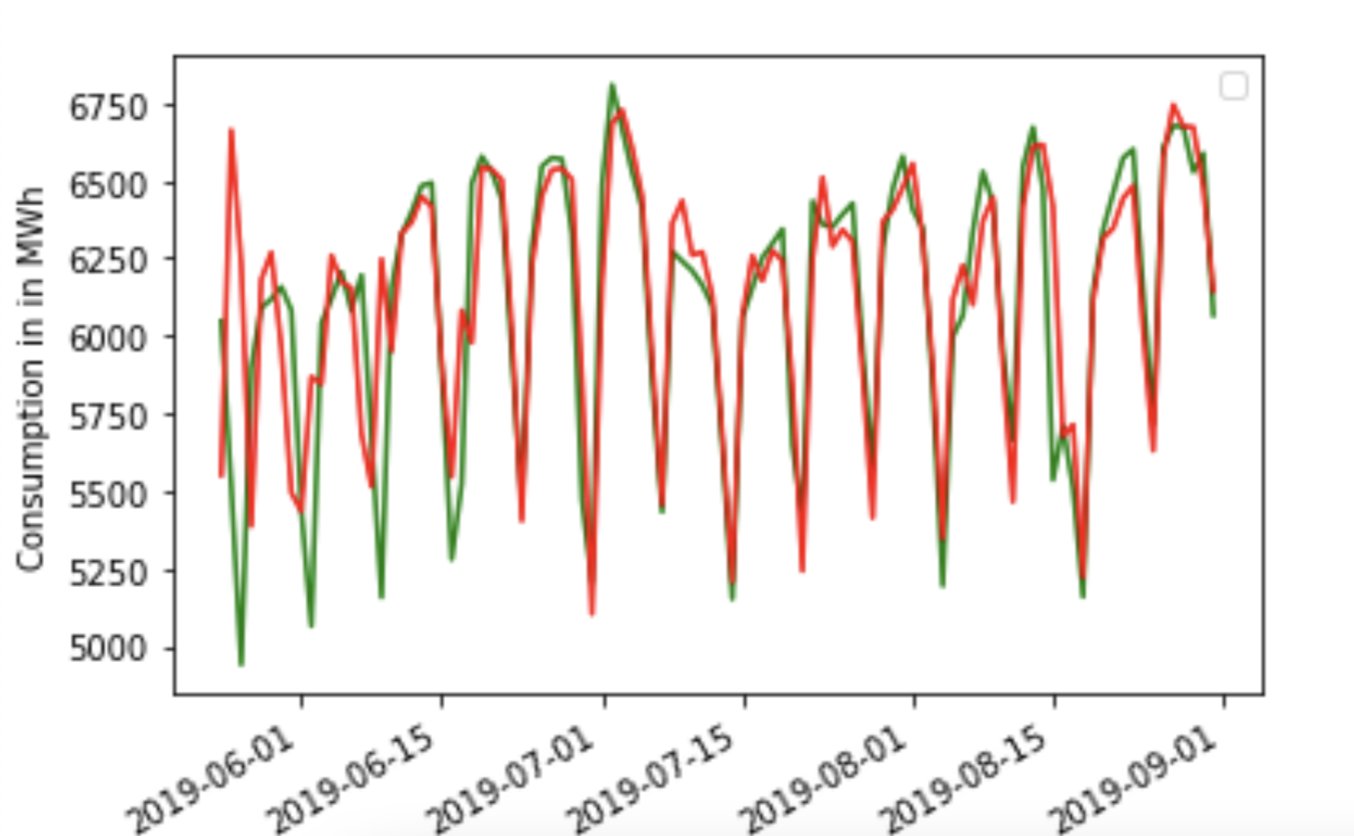
\includegraphics[width=9cm]{final-report-latex/LSTM_Figure.png}
   \caption{LSTM-based RNN model results}
   \end{center}
\end{figure}

Figure 12 offers a sample of the results provided by the LSTM-based RNN. There is only one significant discrepancy that can be observed: the one between 5517 and 6663. This particular divergence is associated with 03-06-2019, a typical weekday of summer in which the electricity load was extremely low. This exception proves that in the absence of weather data, even the best performing deep-learning models cannot predict values that are entirely dependent on weather events. 
\begin{figure}[H]
\begin{center}
   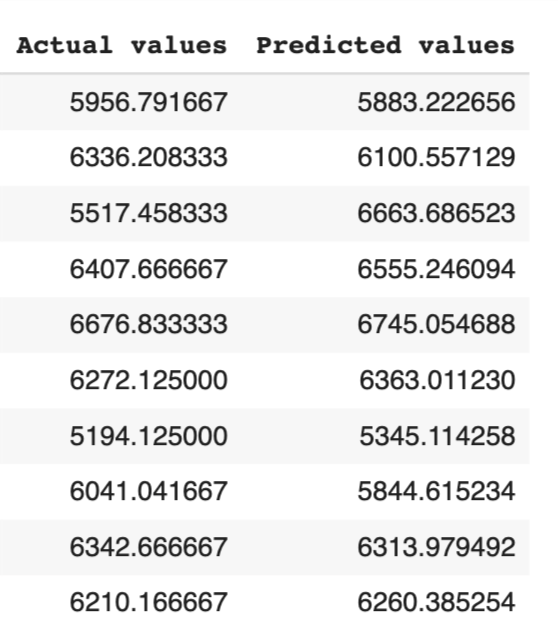
\includegraphics[width=6cm]{final-report-latex/Sample.png}
   \caption{Sample of results}
   \end{center}
\end{figure}


Lastly, figure 13 displays the evolution of the absolute error of the LSTM-based RNN model, defined as the difference between the actual value and the predicted value. One noticeable pattern is that in cases in which the error was very large, it was almost always negative, meaning that the LSTM-based model predicted more consumption. Combined with the negative MBE, this means that for such a model to be useful in industry, grid operators would need to adjust upwardly on average, but also expect that at certain moments the estimations will be massively above the true values in MWh.

\begin{figure}[H]
\begin{center}
   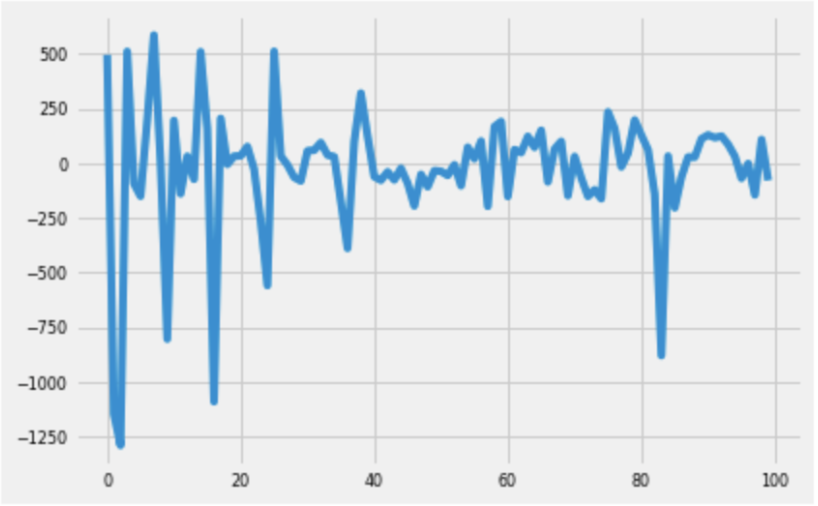
\includegraphics[width=9cm]{final-report-latex/Error.png}
   \caption{Evolution of the error for the LSTM-based RNN}
   \end{center}
\end{figure}



\section{Conclusions}
Our project proves that deep-learning can be effectively and efficiently used for EDF. We developed an LSTM-based RNN model that predicted the electricity consumed hourly for the Romanian market, and obtained results that are significantly better than the ones driven by traditional econometric models like ARIMA. One clear limitation of the proposed LSTM-based RNN model is that we only use the historical time-series as input, and no other weather-related data. In this sense, future research should try to integrate more information on hourly solar irradiation, wind speed level or rainfall.

\section{Contributions}

All the members of the team have contributed towards the project at all stages. In this sense, we shared responsibility between data analysis tasks and writing tasks as equal as possible. 


\begin{thebibliography}{}

\bibitem  EEl-Mouden (2020)
\textit {Electricity consumption}.
https://github.com/drwiiche/electricity-consumption


\bibitem  HHochreiter and Schmidhuber (1997).
\textit {Long Short-Term Memory}.
Neural Computation, 9(8):1735-1780

\bibitem KKelles et al. (2016)
\textit {Extended forecast methods for day-ahead electricity spot prices applying artificial neural networks}. Applied Energy, 162: 218-230.

\bibitem LLago et al.(2018).
\textit{Forecasting spot electricity prices: Deep learning approaches and empirical comparison of traditional algorithms}. 
Applied Energy, 221:386-405.

\bibitem  MMuzaffar and Afshari (2019).
\textit{Short-Term Load Forecasts Using LSTM Networks}. 
Energy Procedia, 158:2922-2927.

\bibitem NNowotarski and Weron (2018)
\textit {Recent advances in electricity price forecasting: A review of probabilistic forecasting} Renewable and Sustainable Energy Reviews, 81:1548-1568

\bibitem   SSon and Kim (2020)
\textit{Predicting Residential Energy Consumption using CNN-LSTM Neural Networks}. 
Energy, 182:72-81.

\bibitem    ZZheng  et  al (2017)
\textit{Electric load forecasting in smart grids using Long-Short-Term-Memory based Recurrent Neural Network}. 
51st Annual Conference on Information Sciences and Systems (CISS).


\end{thebibliography}



\end{document}
